\documentclass[letterpaper,12pt]{article}
\usepackage{tabularx} % extra features for tabular environment
\usepackage{amsmath}  % improve math presentation
\usepackage{graphicx} % takes care of graphic including machinery
\usepackage[margin=0.95in,letterpaper]{geometry} % decreases margins
\usepackage{cite} % takes care of citations
\usepackage[titletoc,title]{appendix} % takes care of appendices
\usepackage{listings} % code representation
\usepackage{pdflscape}
\usepackage{csquotes} % for quoting existing work
\usepackage{color} % defines colors for code listings
\usepackage{comment} % allows for block of comments
\usepackage{gensymb} % degree symbol
\usepackage[final]{hyperref} % adds hyper links inside the generated pdf file

% style code listings
\definecolor{codegreen}{rgb}{0,0.6,0}
\definecolor{codegray}{rgb}{0.5,0.5,0.5}
\definecolor{backcolour}{rgb}{0.95,0.95,0.92}
\lstdefinestyle{mystyle}{
    backgroundcolor=\color{backcolour},   
    commentstyle=\color{codegreen},
    keywordstyle=\color{blue},
    numberstyle=\tiny\color{codegray},
    basicstyle=\footnotesize,
    breakatwhitespace=false,         
    breaklines=true,                 
    captionpos=b,                    
    keepspaces=true,                 
    numbers=left,                    
    numbersep=5pt,                  
    showspaces=false,                
    showstringspaces=false,
    showtabs=false,                  
    tabsize=4
}
\lstset{style=mystyle}

\begin{document}

\title{CS5011 Artificial Intelligence Practice\\Practical 1 Report}
\author{Student ID: 150014151}
\date{11 October, 2019}
\maketitle
\newpage


% --------------------------------------- 1 - INTRODUCTION ------------------------------------------ 

\section{Introduction}
\label{sec:introduction}

The Advanced Agent was attempted for this Practical. The following features were implemented:
\begin{itemize}
    \item Basic Agent:
    \begin{itemize}
       \item Breadth-First Search
        \item Depth-First Search
    \end{itemize}
    \item Intermediate Agent:
    \begin{itemize}
        \item Best-First Search
        \item A* Search
    \end{itemize}
    \item Advanced Agent (1 extension):
    \begin{itemize}
        \item Weather obstacles
    \end{itemize}
\end{itemize}

\subsection{Usage}

\subsubsection{Compilation}

To compile the program, navigate to the \textit{A1src} directory and run the following command:\\

\textit{javac src/A1Main.java}.

\subsubsection{Program Execution}

Once the program has been compiled, it can be executed using the following command:\\

\textit{java A1Main \textless search\_type\textgreater \textless world\_size\textgreater \textless start\_goal\textgreater \textless end\_goal\textgreater [\textless obstacles\textgreater]},\\

where:

\begin{itemize}
    \item \textit{search\_type} is the type of search algorithm used to find a route. It can take the following values: \textit{BFS}, \textit{DFS}, \textit{BestF}, \textit{AStar}. It is written as a String.
    \item \textit{world\_size} is the size of the world, specified by the number of parallels. It is written as a positive integer.
    \item \textit{start\_goal} is the starting point of the flight. It is written as a tuple of positive integers, e.g. \textit{(2,45)}.
    \item \textit{end\_goal} is the goal point that the flight must reach. It is also written as a tuple of positive integers.
    \item \textit{obstacles} is a number of locations in the world that the flight cannot take when looking for a route. They are also written as a tuple of positive integers. There can be any number of obstacles, ranging from 0 to the limit set by the Java Virtual Machine \cite{kabutz2017}.
\end{itemize}

\subsubsection{Examples}

Here are a few examples that can be used to run the program:

\begin{itemize}
    \item Running BFS with no obstacles: \textit{``java A1Main BFS 5 2,45 3,225''}
    \item Running DFS with no obstacles: \textit{``java A1Main DFS 8 1,315 5,270''}
    \item Running BestF with 1 obstacle: \textit{``java A1Main BestF 4 1,45 3,225 1,90''}
    \item Running A* with 2 obstacles: \textit{``java A1Main AStar 4 1,45 3,225 1,90 1,0''}
    \item Running BFS with no possible solution: \textit{``java A1Main BFS 4 1,45 3,225 1,90 1,0 2,45''}
\end{itemize}

% -------------------------- 2 - DESIGN - IMPLEMENTATION - EVALUATION -------------------------------

\newpage
\section{Design, Implementation \& Evaluation}
\label{sec:design-implementation-evaluation}

\subsection{Design \& Implementation}

% ----------------------------------

\subsubsection{PEAS Model}

\paragraph{Performance measure} The path length from initial to goal state, the path cost, the number of states explored, the depth of the tree, the number of nodes created, and the runtime.

\paragraph{Environment} A circular world of size N, which represents the number of parallels. Each parallel is divided in 8 meridians, ranging from 0 to 360 degrees, as depicted in Figure \ref{fig:map}.

\paragraph{Actuators} Moving in of the four following directions, as per Figure \ref{fig:map}: East (H90), South (H180), West (H270) and North (H360).

\paragraph{Sensors} The flight can see in any of the four aforementioned directions from a state in the world. It also knows if the move is valid based on a set of rules specified in Section \ref{sec:problem_definition}.

\begin{figure}[ht]
\centering
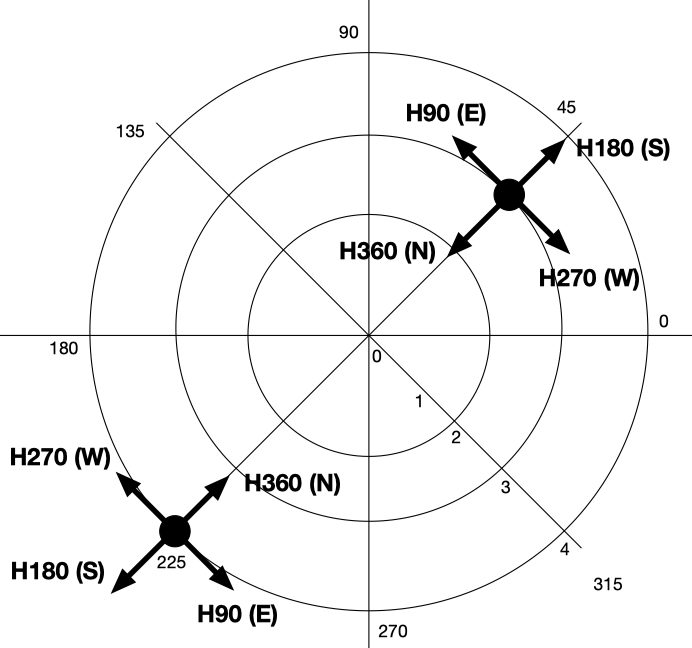
\includegraphics[width=0.5\textwidth]{report/figures/map.png}
\caption{\label{fig:map}A visualisation of a state space and its valid moves where $N=5$.}
\end{figure}

% ----------------------------------

\subsubsection{Problem Definition}
\label{sec:problem_definition}

\paragraph{State space} Corresponds to each position in the map. Each position is represented by a State object, as shown in the UML Class diagram in Appendix \ref{sec:uml_class_diagram}. The state space as a whole is implemented with a \textit{LinkedList} of \textit{LinkesLists} of \textit{Nodes}: \textit{``LinkedList<LinkedList<State>> world''}, as shown in Figure \ref{fig:state_space}.

\begin{figure}[ht]
\centering
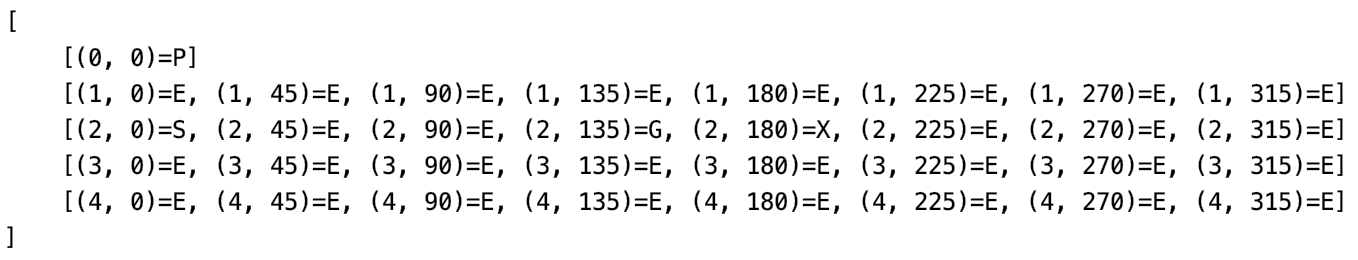
\includegraphics[width=0.8\textwidth]{report/figures/world.png}
\caption{\label{fig:state_space}An example of the implementation of a state space using \textit{LinkedLists} where $N=5$. The initial state $S$ can be seen at \textit{2,0}, the goal state $G$ at \textit{(2,135)}, an obstacle $X$ at \textit{(2,180}) and the pole $P$ at \textit{(0,0)}.}
\end{figure}

\paragraph{Initial State} Corresponds to the starting point defined by the user input, which is used to create the root node of the search tree. For example, in the implementation in Figure \ref{fig:state_space}, the initial state can be found at \textit{(2, 0)=S}. The goal state is stored in the Problem object, as shown in Appendix \ref{sec:uml_class_diagram}. It is impossible to start from the pole (0,0).

\paragraph{Goal} To find the route from the initial state to the goal state while avoiding obstacles. For informed search algorithms, the goal includes finding the route with the minimal path cost. It is impossible for a goal state to be in the pole (0,0). %The goal state is stored in the Problem object, as shown in Appendix \ref{sec:uml_class_diagram}.\\

\paragraph{Successor Function} The successor function (see listing below) generates a set of all the valid nodes that are adjacent to the current node, which are added to an \textit{ArrayList} before being added to the frontier. Additionally, it checks that no invalid moves are added to the \textit{ArrayList}.

\lstinputlisting[label={lst:successor},language=Java]{report/listings/successor.java}

\paragraph{Actions} The flight can move in one of four directions at a time (see Figure \ref{fig:map}). It can move East (H90) by adding 45\degree to its angle, move West (H270) by subtracting 45\degree from its angle, move North (H360) towards the pole (0,0) by subtracting 1 to its current parallel, or move South (H180) towards the extremity of the world by adding 1 to its current parallel. It cannot move to/through the pole \textit{(0,0)}, to a parallel bigger than $N$, or to an obstacle.

\paragraph{Path Cost} Because the state space is a circular map, there are two different costs. The cost to move across parallels ($N \rightarrow N+1$ or $N \rightarrow N-1$) is 1, while the cost to move across meridians ($+45\degree$ or $-45\degree$) is $(2*\pi*d) / 8$. The cost is stored in the \textit{pathCost} of the \textit{Node} class.

% ----------------------------------

\subsubsection{System Architecture}

\paragraph{Class Design}

The system is designed with scalability and simplicity in mind. Therefore, the foundation of the system was built around the general search algorithm (see Figure \ref{fig:general_algorithm}) provided in the lecture slides \cite{generalsearchalg}.

\begin{figure}[ht]
\centering
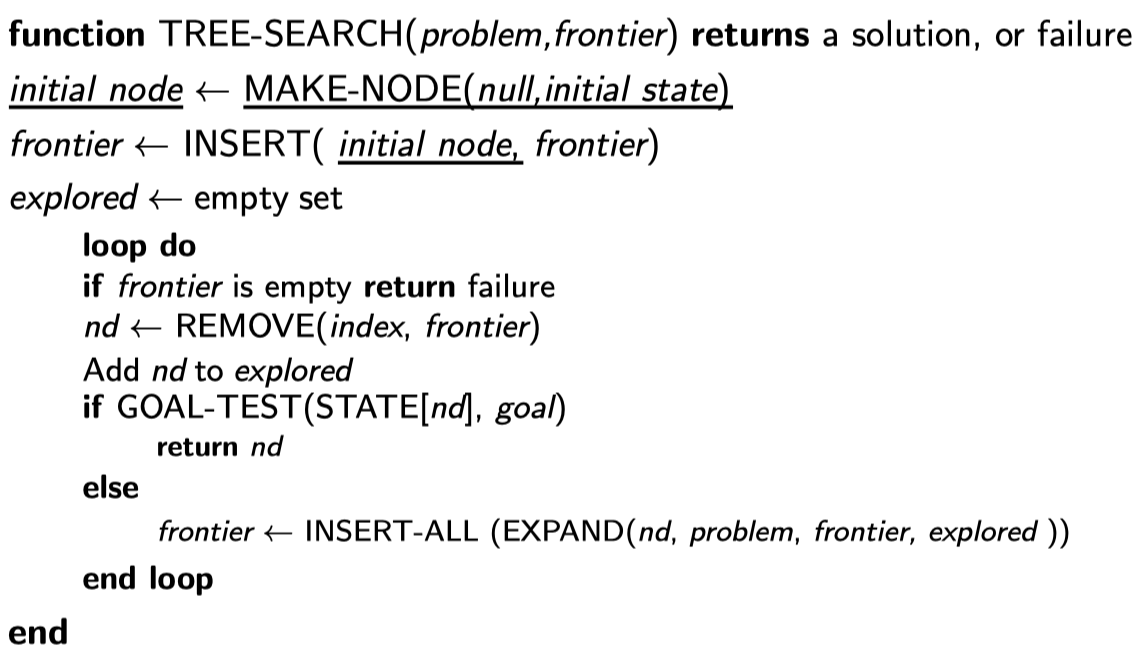
\includegraphics[width=0.7\textwidth]{report/figures/general_search_algorithm.png}
\caption{\label{fig:general_algorithm}The general search algorithm \cite{generalsearchalg}}
\end{figure}

Because the search algorithms implemented share many similarities with the general search algorithm, abstract classes are used to avoid unnecessary code duplication by grouping common methods between the different search algorithms. An overview of the class design can be found in the UML Class Diagram in Appendix \ref{sec:uml_class_diagram}. A top-level abstract class called \textit{GeneralSearch} organises all the general search methods such as \textit{successor()}, \textit{goalTest()}, \textit{isNodeInExploredSet()} or \textit{findSolutionPathCost()} into a single class. Abstract methods, such as \textit{makeNode}, which differ in implementation between informed and uninformed search algorithms, are defined in this class and act as a template to implement in classes that extend \textit{GeneralSearch}.\\

Next, two abstract classes, \textit{InformedSearch} and \textit{UninformedSearch}, extend \textit{GeneralSearch} and its methods. In a similar fashion, they contain methods common to all concrete search algorithms, such as \textit{treeSearch}, \textit{expand} and \textit{removeFrontierNode}. They also override the \textit{makeNode} method declared in the \textit{GeneralSearch} abstract class, and declare their own abstract methods that will be extended by the concrete classes.\\

Finally, concrete classes extending the abstract classes are created. The \textit{BFS} and \textit{DFS} classes extend the \textit{UninformedSearch} abstract class, while the \textit{BestF} and \textit{AStar} classes extend the \textit{InformedSearch} abstract class.

\paragraph{Data Structures}

Java offers a wide variety of data structures to use. The pros and the cons were weighed to choose which data structure to use for each aspect of the program. Concerning the frontier, two data structures are used. For uninformed search, a \textit{LinkedList} is used, while for informed search, a \textit{PriorityQueue} is used. \textit{LinkedLists} are used because manipulation operations for adding/removing Nodes to/from the data structure are much cheaper than \textit{ArrayLists} manipulations \cite{diffLLAL}.\\

Additionally, custom classes are created to easily store and access different aspects of the data. A \textit{Node} object holds crucial information such as:
\begin{itemize}
    \item a pointer to a parent Node, which is used to retrace the route found and to calculate the route's cost,
    \item an action (H90, H180, H270, H360),
    \item a path cost,
    \item a depth,
    \item a \textit{State} (custom class).
\end{itemize}

States represent a location on the state space, including a parallel, an angle, an index to easily access it in the world, and a status to represent if the location is the initial state (S), the goal state (G), the pole (P) or an obstacle (X) (see Figure \ref{fig:map}).

% ----------------------------------

\subsubsection{Uninformed Search}

todo

% ----------------------------------

\subsubsection{Uninformed Search}

todo

% ----------------------------------

\subsubsection{Additional Features}

\paragraph{Invalid Input Security} Robust checks are carried out to ensure that correct arguments are passed when running the program. These include grounding the flight if the initial state S = (0,0) or if the goal state G = (0,0)\footnote{This includes any meridian located on parallel $d=0$ e.g. (0,45) is an invalid location.}.

\paragraph{Javadocs} The entire system is covered by Javadoc \cite{javadoc} comments. They can be compiled using the command below and opening the \textit{javadoc/index.html} file in a web browser:\\

\textit{javadoc -d javadoc A1src/*.java}

% ----------------------------------

\subsection{Evaluation}

todo

\begin{comment}
This section is about performance of the system. A critical analysis of the functionalities of your system and what can be improved. The role of this section is to show and demonstrate the qualities and limitations of your system such as how effectively or efficiently the system works under certain conditions.\\

Depending on the type of assignment, this section should include results of any evaluation performed at a large scale, for example a table/graph showing performance results.\\

Pros and Cons of your approach should also be discussed, and any component that could be improved.\\
\end{comment}

% -------------------------------------- 3 - TEST SUMMARY ------------------------------------------ 
\section{Test Summary}
\label{sec:test-summary}

This section is about correctness of the system. Include a table or a list of tests performed, with input and output where appropriate. The role of this part is to show that your system is working correctly. You could also include:

\begin{itemize}
    \item Screenshots of the outputs
    \item Small working examples
    \item Graphical representation of these working examples (etc)
\end{itemize}

% -------------------------------------------- APPENDIX -------------------------------------------- 

\newpage
\begin{appendices}

\section{UML Class Diagram}
\label{sec:uml_class_diagram}

The UML Class Diagram of the program, generated using yWorks \cite{yworks}.

\begin{figure}[ht]
\centering
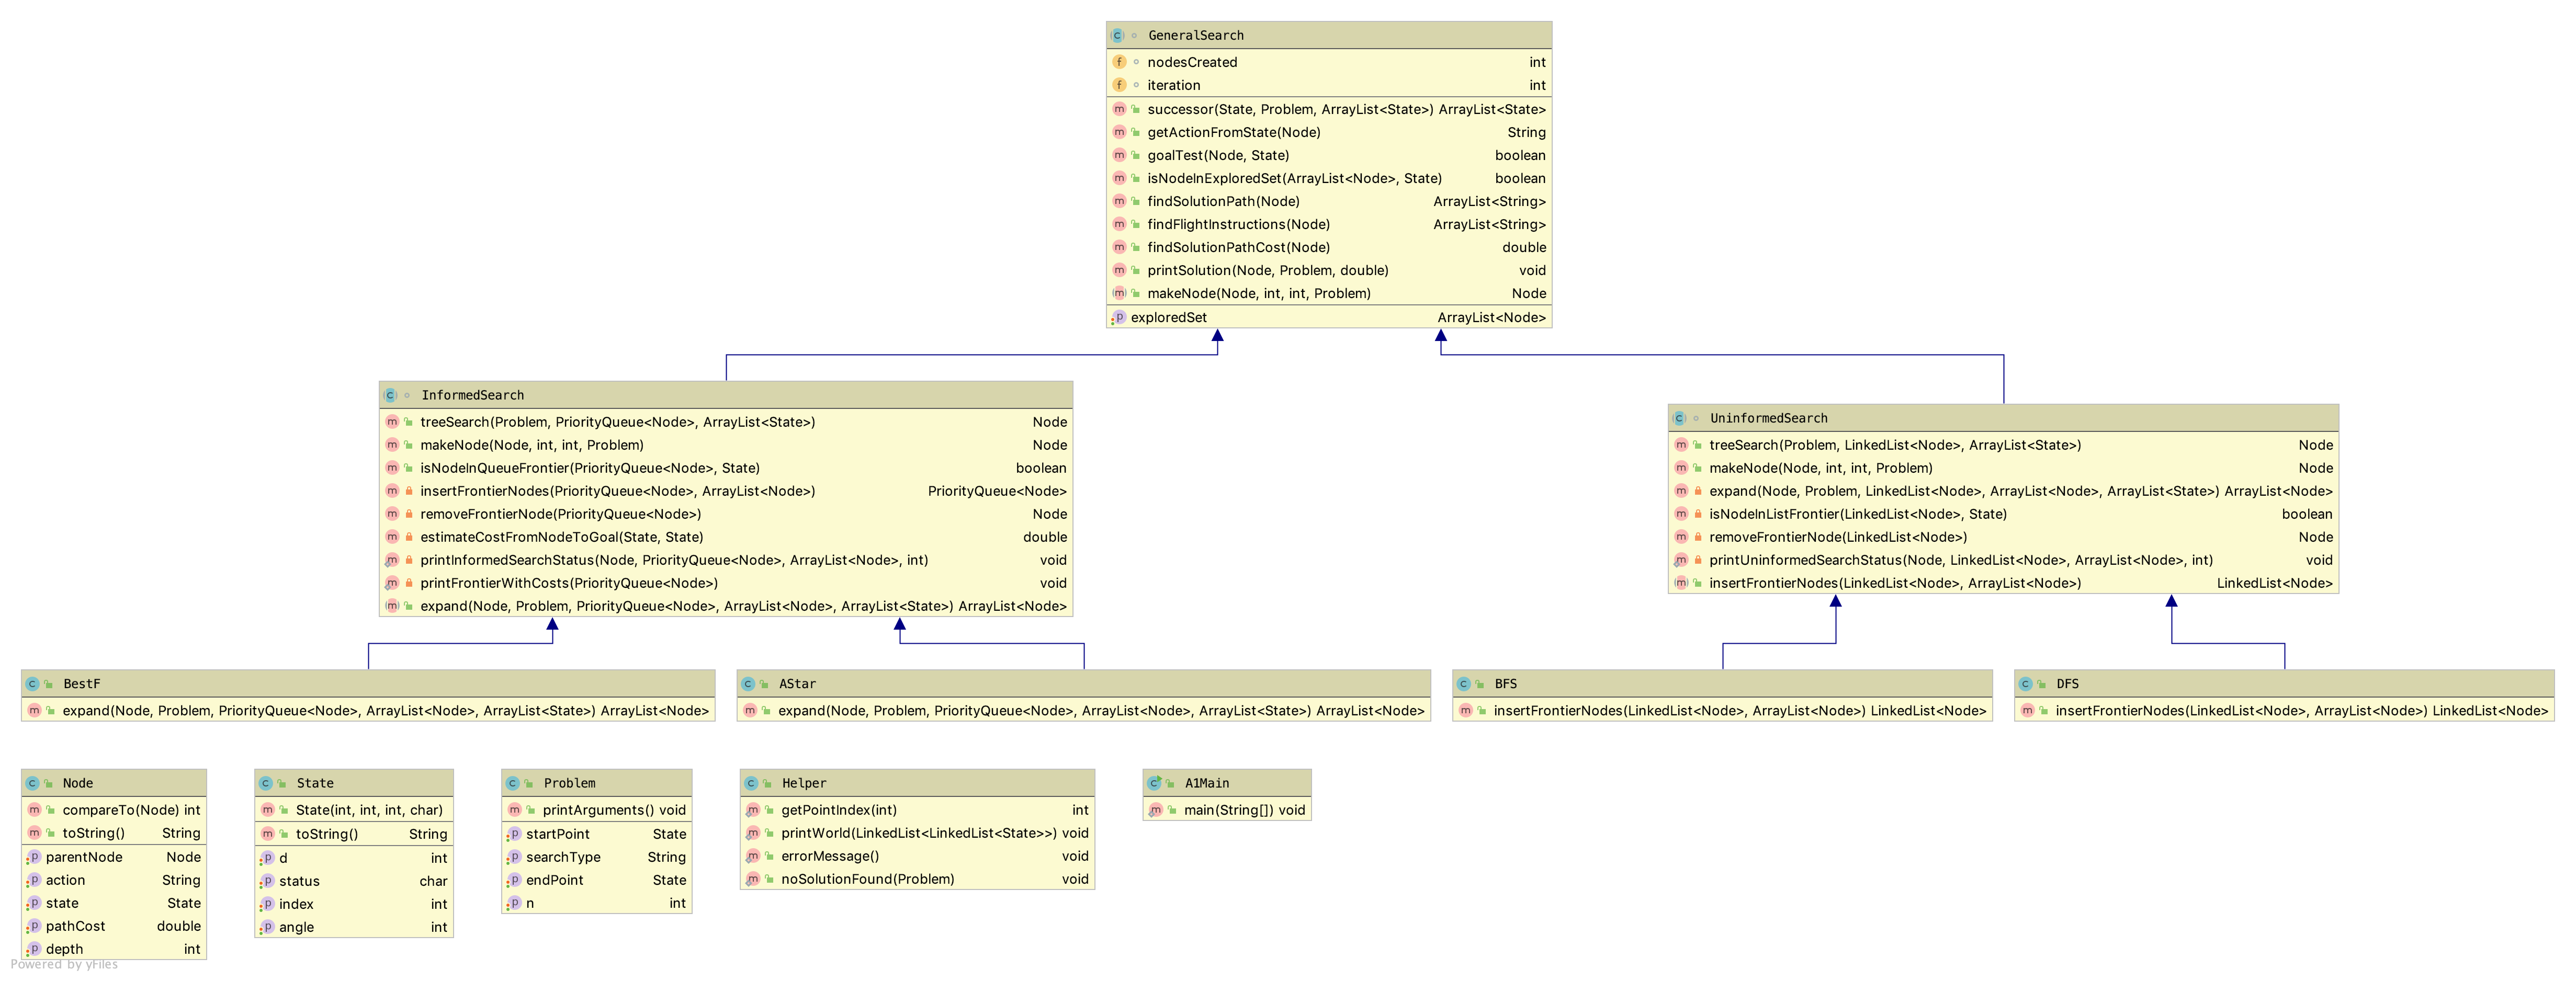
\includegraphics[width=0.99\textwidth]{UML/UML_class_diagram.png}
{\label{fig:uml_class_diagram}}
\end{figure}

\newpage
\section{Path length across different algorithms}
\label{sec:appendix-path-length}
\begin{table}[ht]
\centering
\begin{tabular}{r|c|c|c|c|}
\cline{2-5}
\multicolumn{1}{l|}{} & \textbf{BFS} & \textbf{DFS} & \textbf{BestF} & \textbf{A*} \\ \hline
\multicolumn{1}{|r|}{\textit{i. N=5 S=(2,0) G=(2,135)}} & 3 & 3 & 3 & 5 \\ \hline
\multicolumn{1}{|r|}{\textit{ii. N=5 S=(1,180) G=(4,180)}} & 3 & 11 & 3 & 3 \\ \hline
\multicolumn{1}{|r|}{\textit{iii. N=5 S=(1,315) G=(4,45)}} & 5 & 13 & 5 & 11 \\ \hline
\multicolumn{1}{|r|}{\textit{v. N=8 S=(1,135) G=(5,315)}} & 4 & 20 & 4 & 4 \\ \hline
\multicolumn{1}{|r|}{\textit{vi. N=8 S=(4,0) G=(7,90)}} & 5 & 13 & 5 & 5 \\ \hline
\multicolumn{1}{|r|}{\textit{viii. N=10 S=(9,225) G=(2,45)}} & 11 & 35 & 13 & 15 \\ \hline
\multicolumn{1}{|r|}{\textit{ix. N=10 S=(2,45) G=(9,225)}} & 11 & 35 & 11 & 15 \\ \hline
\multicolumn{1}{|r|}{\textit{x. N=10 S=(7,270) G=(7,90)}} & 4 & 4 & 16 & 18 \\ \hline
\end{tabular}
\caption{Path length}
\label{tab:path_length}
\end{table}

\section{Path cost across different algorithms}
\label{sec:appendix-path-cost}
\begin{table}[ht]
\centering
\begin{tabular}{r|c|c|c|c|}
\cline{2-5}
\multicolumn{1}{l|}{} & \textbf{BFS} & \textbf{DFS} & \textbf{BestF} & \textbf{A*} \\ \hline
\multicolumn{1}{|r|}{\textit{i. N=5 S=(2,0) G=(2,135)}} & 4.712 & 4.712 & 4.712 & 5.142 \\ \hline
\multicolumn{1}{|r|}{\textit{ii. N=5 S=(1,180) G=(4,180)}} & 3 & 11.639 & 3 & 3 \\ \hline
\multicolumn{1}{|r|}{\textit{iii. N=5 S=(1,315) G=(4,45)}} & 4.571 & 16.352 & 8.498 & 5.785 \\ \hline
\multicolumn{1}{|r|}{\textit{v. N=8 S=(1,135) G=(5,315)}} & 4 & 35.416 & 4 & 4 \\ \hline
\multicolumn{1}{|r|}{\textit{vi. N=8 S=(4,0) G=(7,90)}} & 9.283 & 39.914 & 9.283 & 9.283 \\ \hline
\multicolumn{1}{|r|}{\textit{viii. N=10 S=(9,225) G=(2,45)}} & 35.274 & 135.805 & 24.708 & 11 \\ \hline
\multicolumn{1}{|r|}{\textit{ix. N=10 S=(2,45) G=(9,225)}} & 13.283 & 120.097 & 13.283 & 12.571 \\ \hline
\multicolumn{1}{|r|}{\textit{x. N=10 S=(7,270) G=(7,90)}} & 21.991 & 21.991 & 19.854 & 15.571 \\ \hline
\end{tabular}
\caption{Path cost}
\label{tab:path_cost}
\end{table}

\newpage
\section{Numbers of nodes expanded across different algorithms}
\label{sec:appendix-nodes-expanded}
\begin{table}[ht]
\centering
\begin{tabular}{r|c|c|c|c|}
\cline{2-5}
\multicolumn{1}{l|}{} & \textbf{BFS} & \textbf{DFS} & \textbf{BestF} & \textbf{A*} \\ \hline
\multicolumn{1}{|r|}{\textit{i. N=5 S=(2,0) G=(2,135)}} & 13 & 4 & 4 & 13 \\ \hline
\multicolumn{1}{|r|}{\textit{ii. N=5 S=(1,180) G=(4,180)}} & 21 & 25 & 7 & 9 \\ \hline
\multicolumn{1}{|r|}{\textit{iii. N=5 S=(1,315) G=(4,45)}} & 33 & 23 & 28 & 26 \\ \hline
\multicolumn{1}{|r|}{\textit{v. N=8 S=(1,135) G=(5,315)}} & 30 & 23 & 9 & 11 \\ \hline
\multicolumn{1}{|r|}{\textit{vi. N=8 S=(4,0) G=(7,90)}} & 44 & 46 & 9 & 11 \\ \hline
\multicolumn{1}{|r|}{\textit{viii. N=10 S=(9,225) G=(2,45)}} & 72 & 36 & 24 & 38 \\ \hline
\multicolumn{1}{|r|}{\textit{ix. N=10 S=(2,45) G=(9,225)}} & 79 & 45 & 22 & 37 \\ \hline
\multicolumn{1}{|r|}{\textit{x. N=10 S=(7,270) G=(7,90)}} & 25 & 5 & 30 & 43 \\ \hline
\end{tabular}
\caption{Nodes/States Expanded			}
\label{tab:nodes-expanded}
\end{table}

\section{Runtime across different algorithms}
\label{sec:appendix-runtime}
\begin{table}[ht]
\centering
\begin{tabular}{r|c|c|c|c|}
\cline{2-5}
\multicolumn{1}{l|}{} & \textbf{BFS} & \textbf{DFS} & \textbf{BestF} & \textbf{A*} \\ \hline
\multicolumn{1}{|r|}{\textit{i. N=5 S=(2,0) G=(2,135)}} & 3.684 & 2.64 & 7.166 & 8.07 \\ \hline
\multicolumn{1}{|r|}{\textit{ii. N=5 S=(1,180) G=(4,180)}} & 5.606 & 6.977 & 5.975 & 6.858 \\ \hline
\multicolumn{1}{|r|}{\textit{iii. N=5 S=(1,315) G=(4,45)}} & 7.841 & 5.817 & 14.596 & 11.578 \\ \hline
\multicolumn{1}{|r|}{\textit{v. N=8 S=(1,135) G=(5,315)}} & 8.881 & 6.08 & 7.257 & 7.489 \\ \hline
\multicolumn{1}{|r|}{\textit{vi. N=8 S=(4,0) G=(7,90)}} & 11.234 & 10.708 & 6.744 & 9.283 \\ \hline
\multicolumn{1}{|r|}{\textit{viii. N=10 S=(9,225) G=(2,45)}} & 11.658 & 8.161 & 14.814 & 15.223 \\ \hline
\multicolumn{1}{|r|}{\textit{ix. N=10 S=(2,45) G=(9,225)}} & 13.42 & 8.852 & 12.803 & 14.164 \\ \hline
\multicolumn{1}{|r|}{\textit{x. N=10 S=(7,270) G=(7,90)}} & 21.991 & 2.948 & 19.296 & 17.119 \\ \hline
\end{tabular}
\caption{Runtime (ms)}
\label{tab:runtime}
\end{table}

\newpage
\section{Node depth across different algorithms}
\label{sec:appendix-node-depth}
\begin{table}[ht]
\centering
\begin{tabular}{r|c|c|c|c|}
\cline{2-5}
\multicolumn{1}{l|}{} & \textbf{BFS} & \textbf{DFS} & \textbf{BestF} & \textbf{A*} \\ \hline
\multicolumn{1}{|r|}{\textit{i. N=5 S=(2,0) G=(2,135)}} & 3 & 3 & 3 & 5 \\ \hline
\multicolumn{1}{|r|}{\textit{ii. N=5 S=(1,180) G=(4,180)}} & 3 & 11 & 3 & 3 \\ \hline
\multicolumn{1}{|r|}{\textit{iii. N=5 S=(1,315) G=(4,45)}} & 5 & 13 & 5 & 11 \\ \hline
\multicolumn{1}{|r|}{\textit{v. N=8 S=(1,135) G=(5,315)}} & 4 & 20 & 4 & 4 \\ \hline
\multicolumn{1}{|r|}{\textit{vi. N=8 S=(4,0) G=(7,90)}} & 5 & 13 & 5 & 5 \\ \hline
\multicolumn{1}{|r|}{\textit{viii. N=10 S=(9,225) G=(2,45)}} & 11 & 35 & 13 & 15 \\ \hline
\multicolumn{1}{|r|}{\textit{ix. N=10 S=(2,45) G=(9,225)}} & 11 & 35 & 11 & 15 \\ \hline
\multicolumn{1}{|r|}{\textit{x. N=10 S=(7,270) G=(7,90)}} & 4 & 4 & 16 & 18 \\ \hline
\end{tabular}
\caption{Node depth}
\label{tab:node_depth}
\end{table}

\section{Number of nodes created across different algorithms}
\label{sec:appendix-nodes-created}
\begin{table}[ht]
\centering
\begin{tabular}{r|c|c|c|c|}
\cline{2-5}
\multicolumn{1}{l|}{} & \textbf{BFS} & \textbf{DFS} & \textbf{BestF} & \textbf{A*} \\ \hline
\multicolumn{1}{|r|}{\textit{i. N=5 S=(2,0) G=(2,135)}} & 22 & 11 & 11 & 47 \\ \hline
\multicolumn{1}{|r|}{\textit{ii. N=5 S=(1,180) G=(4,180)}} & 30 & 39 & 16 & 33 \\ \hline
\multicolumn{1}{|r|}{\textit{iii. N=5 S=(1,315) G=(4,45)}} & 37 & 39 & 37 & 26 \\ \hline
\multicolumn{1}{|r|}{\textit{v. N=8 S=(1,135) G=(5,315)}} & 38 & 45 & 20 & 40 \\ \hline
\multicolumn{1}{|r|}{\textit{vi. N=8 S=(4,0) G=(7,90)}} & 55 & 63 & 22 & 41 \\ \hline
\multicolumn{1}{|r|}{\textit{viii. N=10 S=(9,225) G=(2,45)}} & 76 & 65 & 46 & 136 \\ \hline
\multicolumn{1}{|r|}{\textit{ix. N=10 S=(2,45) G=(9,225)}} & 79 & 79 & 46 & 135 \\ \hline
\multicolumn{1}{|r|}{\textit{x. N=10 S=(7,270) G=(7,90)}} & 36 & 14 & 56 & 162 \\ \hline
\end{tabular}
\caption{Nodes created}
\label{tab:nodes_created}
\end{table}

\newpage
\bibliographystyle{plain}
\bibliography{bibliography}

\end{appendices}
\end{document}